\begin{enumerate}[label=\thechapter.\arabic*,ref=\thechapter.\theenumi]
    \item The Fourier transform X\brak{j\omega} of the signal\\ $x(t)=\frac{t}{\brak{1+t^2}^2}$ is \rule{1.5cm}{0.15mm}.\hfill{GATE-2022-EC-15}
\begin{enumerate}
	\item[(A)] $\frac{\pi}{2j}\omega e^{-\abs{\omega}}$
	\item[(B)] $\frac{\pi}{2}\omega e^{-\abs{\omega}}$
	\item[(C)] $\frac{\pi}{2j}e^{-\abs{\omega}}$
	\item[(D)] $\frac{\pi}{2}e^{-\abs{\omega}}$
\end{enumerate}

\solution
% \iffalse
\let\negmedspace\undefined
\let\negthickspace\undefined
\documentclass[journal,12pt,twocolumn]{IEEEtran}
\usepackage{cite}
\usepackage{amsmath,amssymb,amsfonts,amsthm}
\usepackage{algorithmic}
\usepackage{graphicx}
\usepackage{textcomp}
\usepackage{xcolor}
\usepackage{txfonts}
\usepackage{listings}
\usepackage{enumitem}
\usepackage{mathtools}
\usepackage{gensymb}
\usepackage{comment}
\usepackage[breaklinks=true]{hyperref}
\usepackage{tkz-euclide} 
\usepackage{listings}
\usepackage{gvv}                                        
\def\inputGnumericTable{}                                 
\usepackage[latin1]{inputenc}                                
\usepackage{color}                                            
\usepackage{array}                                            
\usepackage{longtable}                                       
\usepackage{calc}                                             
\usepackage{multirow}                                         
\usepackage{hhline}                                           
\usepackage{ifthen}                                           
\usepackage{lscape}

\makeatletter

\newcommand*{\underarrow}{\def\@underarrow{\relax}\@ifstar{\@@underarrow}{\def\@underarrow{\hidewidth}\@@underarrow}}
\newcommand*{\@@underarrow}[2][]{\underset{\@underarrow\substack{\uparrow\if\relax\detokenize{#1}\relax\else\\#1\fi}\@underarrow}{#2}}

\newcommand*{\overarrow}{\def\@overarrow{\relax}\@ifstar{\@@overarrow}{\def\@overarrow{\hidewidth}\@@overarrow}}
\newcommand*{\@@overarrow}[2][]{\overset{\@overarrow\substack{\if\relax\detokenize{#1}\relax\else#1\\\fi\downarrow}\@overarrow}{#2}}
\makeatother
\newtheorem{theorem}{Theorem}[section]
\newtheorem{problem}{Problem}
\newtheorem{proposition}{Proposition}[section]
\newtheorem{lemma}{Lemma}[section]
\newtheorem{corollary}[theorem]{Corollary}
\newtheorem{example}{Example}[section]
\newtheorem{definition}[problem]{Definition}
\newcommand{\BEQA}{\begin{eqnarray}}
\newcommand{\EEQA}{\end{eqnarray}}
\newcommand{\define}{\stackrel{\triangle}{=}}
\theoremstyle{remark}
\newtheorem{rem}{Remark}
\begin{document}
\parindent 0px

\bibliographystyle{IEEEtran}
\vspace{3cm}

\title{Assignment\\[1ex]GATE-EE-50}
\author{EE23BTECH11034 - Prabhat Kukunuri$^{}$% <-this % stops a space
}
\maketitle
\newpage
\bigskip

\renewcommand{\thefigure}{\theenumi}
\renewcommand{\thetable}{\theenumi}
\section{Question}
The Fourier transform X\brak{j\omega} of the signal\\ $x(t)=\frac{t}{\brak{1+t^2}^2}$ is \rule{1.5cm}{0.15mm}.
\begin{enumerate}
	\item[(A)] $\frac{\pi}{2j}\omega e^{-\abs{\omega}}$
	\item[(B)] $\frac{\pi}{2}\omega e^{-\abs{\omega}}$
	\item[(C)] $\frac{\pi}{2j}e^{-\abs{\omega}}$
	\item[(D)] $\frac{\pi}{2}e^{-\abs{\omega}}$
\end{enumerate}
\solution
\begin{table}[h]
    \centering
    \begin{tabular}{|p{2cm}|p{2.80cm}|p{2.70cm}|}
    \hline
    Symbol&Value&Description\\ \hline
    $$x(t)$$&$$\frac{t}{\brak{1+t^2}^2}$$&$$\text{Signal}$$\\\hline
    $$X\brak{\omega}$$&$$\int_{t=-\infty}^{\infty}x\brak{t}e^{-j\omega t}dt$$& Fourier transform of $x\brak{t}$\\\hline
    \end{tabular}
    \caption{Variable description}
    \label{tab:GATE-2022-15-1}
\end{table}\\
The Fourier transform of the form x\brak{t}=$e^{-a\abs{t}}$ is 
\begin{align}
    x\brak{t}&\xleftrightarrow{\text{F.T}} X\brak{\omega}\\
    X\brak{\omega}&= \frac{2a}{a^2+\omega^2}
\end{align}
Consider, 
\begin{align}
    x\brak{t}&=e^{-\abs{t}}\\
    X\brak{\omega}&=\frac{2}{1+\omega^2}
\end{align}
By using differentiation property from \eqref{eq:Differentiation-property},
\begin{align}
    tx\brak{t}&\xleftrightarrow{\text{F.T}}j\frac{d}{d\omega}X\brak{\omega}\\
     tx\brak{t}&\xleftrightarrow{\text{F.T}}j\sbrak{\frac{d}{d\omega}\brak{\frac{2}{1+\omega^2}}}\\
     te^{-\abs{t}}&\xleftrightarrow{\text{F.T}}\frac{-4j\omega}{\brak{1+\omega^2}^2}
\end{align}
Applying duality property from \eqref{eq:Duality-property},
\begin{align}
    \frac{-4jt}{\brak{1+t^2}^2}&\xleftrightarrow{\text{F.T}}2\pi\brak{-\omega}e^{-\abs{-\omega}}\\
    \frac{t}{\brak{1+t^2}^2}&\xleftrightarrow{\text{F.T}}\frac{-2\pi\omega e^{-\abs{\omega}}}{-4j}\\
    \frac{t}{\brak{1+t^2}^2}&\xleftrightarrow{\text{F.T}}\frac{\pi}{2j}\omega e^{-\abs{\omega}}
\end{align}
\end{document}

\pagebreak

\item For a vector $\bar{x} = [x[0], x[1], \dots, x[7] ]$, the $8$-point discrete Fourier transform (DFT) is denoted by $\bar{X} = \text{DFT}(\bar{x}) = [X[0],X[1],\dots,X[7]]$, where
    \begin{align*}
    X[k] = \sum_{n=0}^{7}x[n]\exp\left(-j\frac{2\pi}{8}nk\right).
    \end{align*} 
    Here $j = \sqrt{-1}$. If $\bar{x} = [1,0,0,0,2,0,0,0]$ and $\bar{y} = \text{DFT}(\text{DFT}(\bar{x}))$, then the value of $y[0]$ is.\hfill{GATE-2022-EC-55}\\
    \solution
    \iffalse
\documentclass[journal,12pt,onecolumn]{IEEEtran}
\usepackage{cite}
\usepackage{amsmath,amssymb,amsfonts,amsthm}
\usepackage{algorithmic}
\usepackage{graphicx}
\usepackage{textcomp}
\usepackage{xcolor}
\usepackage{txfonts}
\usepackage{listings}
\usepackage{enumitem}
\usepackage{mathtools}
\usepackage{gensymb}
\usepackage{comment}
\usepackage[breaklinks=true]{hyperref}
\usepackage{tkz-euclide}
\usepackage{listings}
\usepackage{gvv}
\def\inputGnumericTable{}
\usepackage[latin1]{inputenc}
\usepackage{color}
\usepackage{array}
\usepackage{longtable}
\usepackage{calc}
\usepackage{multirow}
\usepackage{hhline}
\usepackage{ifthen}
\usepackage{lscape}

\newtheorem{theorem}{Theorem}[section]
\newtheorem{problem}{Problem}
\newtheorem{proposition}{Proposition}[section]
\newtheorem{lemma}{Lemma}[section]
\newtheorem{corollary}[theorem]{Corollary}
\newtheorem{example}{Example}[section]
\newtheorem{definition}[problem]{Definition}
\newcommand{\BEQA}{\begin{eqnarray}}
    \newcommand{\EEQA}{\end{eqnarray}}
\newcommand{\define}{\stackrel{\triangle}{=}}
\theoremstyle{remark}
\newtheorem{rem}{Remark}

\begin{document}
    
    \bibliographystyle{IEEEtran}
    \vspace{3cm}
    
    \title{Gate 2022 EC Q55}
    \author{EE23BTECH11212 - Manugunta Meghana Sai$^{*}$% <-this % stops a space
    }
    \maketitle
    \bigskip
    
    \renewcommand{\thefigure}{\theenumi}
    \renewcommand{\thetable}{\theenumi}
    
    \vspace{3cm}
    \textbf{Gate 2022 EE Q55} 
    
    For a vector $\bar{x} = [x[0], x[1], \dots, x[7] ]$, the $8$-point discrete Fourier transform (DFT) is denoted by $\bar{X} = \text{DFT}(\bar{x}) = [X[0],X[1],\dots,X[7]]$, where
    \begin{align*}
    X[k] = \sum_{n=0}^{7}x[n]\exp\left(-j\frac{2\pi}{8}nk\right).
    \end{align*} 
    Here $j = \sqrt{-1}$. If $\bar{x} = [1,0,0,0,2,0,0,0]$ and $\bar{y} = \text{DFT}(\text{DFT}(\bar{x}))$, then the value of $y[0]$ is\\
    \solution
    \fi
    \begin{table}[h!]
 	\centering
 	\resizebox{6 cm}{!}{
 		\begin{tabular}{|c|c|c|}
	\hline
	\textbf{Parameter} &  \textbf{Description} & \textbf{Value}\\[6pt]
	\hline
	$\bar{X}$ & $\text{DFT}(\bar{x})$ & $-$ \\[6pt]
	\hline
	$\bar{x}$ & vector & $[1,0,0,0,2,0,0,0]$ \\[6pt]
	\hline
	$\bar{y}$ & $\text{DFT}(\text{DFT}(\bar{x}))$ & $-$ \\[6pt]
	\hline 
\end{tabular}

 	}
 	\caption{Given Parameters}
 	\label{tab:msmECgate55tab1} 
 \end{table} 
    \\DFT of $\bar{x}$
    \begin{align}
    X[k] = \sum_{n=0}^{7}x[n]\exp\left(-j\frac{2\pi}{8}nk\right)
    \end{align}
    As the only non-zero values in x are x[0] and x[4]:
    \begin{align}
    X[k] = x[0] + x[4]\exp\left(-j\pi k\right)
    \end{align}
    After substituting the values of k ranging from $0$ to $7$,
    \begin{align}
    \bar{X} &= \text{DFT}(\bar{x}) = [X[0],X[1],\dots,X[7]]\\
    \bar{X} &= [3,-1,3,-1,3,-1,3,-1]
    \end{align}
    \begin{align}
    \bar{y} &= \text{DFT}(\text{DFT}(\bar{x}))\\
    \bar{y} &= [3,-1,3,-1,3,-1,3,-1]\\
    y[0] &= \sum_{n=0}^{7}x[n]\\
    &= x[0] + x[1] + \dots + x[7]\\
    &= 3 -1 +3 -1 +3 -1 +3 -1 = 8
    \end{align}
%\end{document}


    \pagebreak
\item \textbf{Question:} An LTI system is shown in the figure where $$H\brak{s}= \frac{100}{s^2+0.1s+10}$$ The steady state output of the system for an input $x\brak{t}$ is given by $y\brak{t}=a+b\sin{\brak{10t+\theta}}$. The values of $'a'$ and $'b'$ are \\\\
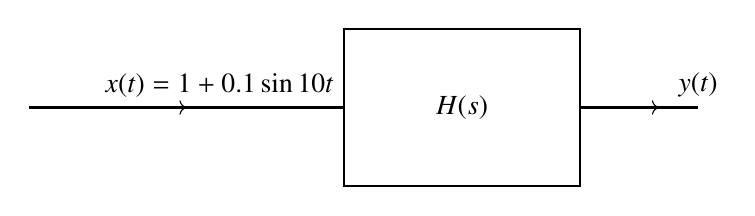
\begin{tikzpicture}
    \draw [thick, draw=black] (-2,-1) -- (2,-1) node[anchor=south east] {$x(t)=1+0.1\sin{\brak{10t}}$};
    \draw [thick,draw=black] (2,0) rectangle (5,-2) ;
    \draw [thick,draw=black] (5,-1) -- (6.5,-1) node[anchor=south] {$y(t)$};
    \draw [->] (-2,-1)--(0,-1);
    \draw [->] (5,-1)--(6,-1);
    \draw (3.5, -1) node[] {$H(s)$};
\end{tikzpicture}\\
\solution 
    \iffalse
\let\negmedspace\undefined
\let\negthickspace\undefined
\documentclass[journal,12pt,twocolumn]{IEEEtran}
\usepackage{cite}
\usepackage{amsmath,amssymb,amsfonts,amsthm}
\usepackage{algorithmic}
\usepackage{graphicx}
\usepackage{textcomp}
\usepackage{xcolor}
\usepackage{txfonts}
\usepackage{listings}
\usepackage{enumitem}
\usepackage{mathtools}
\usepackage{gensymb}
\usepackage{comment}
\usepackage[breaklinks=true]{hyperref}
\usepackage{tkz-euclide} 
\usepackage{listings}
\usepackage{gvv}                                        
%\def\inputGnumericTable{}                                 
\usepackage[latin1]{inputenc}                                
\usepackage{color}                                            
\usepackage{array}                                            
\usepackage{longtable}                                       
\usepackage{calc}                                             
\usepackage{multirow}                                         
\usepackage{hhline}                                           
\usepackage{ifthen}                                           
\usepackage{lscape}
\usepackage{tabularx}
\usepackage{array}
\usepackage{float}


\newtheorem{theorem}{Theorem}[section]
\newtheorem{problem}{Problem}
\newtheorem{proposition}{Proposition}[section]
\newtheorem{lemma}{Lemma}[section]
\newtheorem{corollary}[theorem]{Corollary}
\newtheorem{example}{Example}[section]
\newtheorem{definition}[problem]{Definition}
\newcommand{\BEQA}{\begin{eqnarray}}
\newcommand{\EEQA}{\end{eqnarray}}
\newcommand{\define}{\stackrel{\triangle}{=}}
\theoremstyle{remark}
\newtheorem{rem}{Remark}
\begin{document}

\bibliographystyle{IEEEtran}
\vspace{3cm}

\title{Question 37, EE Gate 2022}
\author{EE23BTECH11017 - Eachempati Mihir Divyansh$^{*}$}
\maketitle
\newpage
\bigskip

\renewcommand{\thefigure}{\theenumi}
\renewcommand{\thetable}{\theenumi}
\textbf{Question:} An LTI system is shown in the figure where $$H\brak{s}= \frac{100}{s^2+0.1s+10}$$ The steady state output of the system for an input $x\brak{t}$ is given by $y\brak{t}=a+b\sin{\brak{10t+\theta}}$. The values of $'a'$ and $'b'$ are \\\\
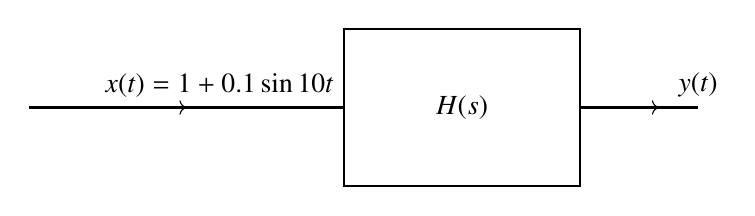
\begin{tikzpicture}
    \draw [thick, draw=black] (-2,-1) -- (2,-1) node[anchor=south east] {$x(t)=1+0.1\sin{\brak{10t}}$};
    \draw [thick,draw=black] (2,0) rectangle (5,-2) ;
    \draw [thick,draw=black] (5,-1) -- (6.5,-1) node[anchor=south] {$y(t)$};
    \draw [->] (-2,-1)--(0,-1);
    \draw [->] (5,-1)--(6,-1);
    \draw (3.5, -1) node[] {$H(s)$};
\end{tikzpicture}

\solution \\
\fi
\begin{table}[h]
    \centering
    \begin{tabular}{|c|c|c|}
    \hline
   Symbol & Value & Description \\
    \hline
    $x\brak{t}$ & $1+0.1\sin{\brak{10t}}$ & Input Signal\\ [2ex]
    \hline
    $y\brak{t}$ & ? & Output of the system\\[2ex]
    \hline 
    $H\brak{s}$ & $\frac{100}{s^2+0.1s+10}$ & Impulse Response\\[2ex]
    \hline
\end{tabular}
    \caption{Given Information} 
    \label{37.Gate22.EE.tab: 1}                                                                                                                                                                                                 
\end{table}
\begin{enumerate}
\item \textbf{Theory: } If a sinusoidal input is given to a system, whose transfer function is known, the output can be calculated as follows
\begin{align}
    y(t)&=h(t)*x(t)\\
    Y(s)&=H(s)X(s)
\end{align}
Let $s=j\omega$
\begin{align}
    Y(j\omega)&=H(j\omega)X(j\omega)
\end{align}
If $\Phi$ is the phase of $H(j\omega)$, 
\begin{align}
    H(j\omega)=\abs{H(j\omega)}e^{j\Phi(\omega)}
\end{align}
If $x(t)=\cos{(\omega_0t)}$, 
\begin{align}
    X(j\omega)&=\pi \brak{\delta(\omega-\omega_0)+\delta(\omega+\omega_0)}
   % \implies X(f)&=\frac{1}{2}\brak{\delta(f-f_0)+\delta(f+f_0)}
\end{align}
Now,
\begin{align}
    Y(j\omega)=&\brak{\delta(\omega-\omega_0)+\delta(\omega+\omega_0)}\abs{H(j\omega)}e^{j\Phi(\omega)}\\
\end{align}
Since $\abs{H(j\omega)}\delta(\omega-\omega_0)$ is zero everywhere except at $\omega_0$ 
\begin{align}
    Y(j\omega)=&\abs{H(j\omega_0)}e^{j\Phi(\omega_0)}\delta(\omega-\omega_0) \\&+ \abs{H(-j\omega_0)}e^{j\Phi(-j\omega_0)}\delta(\omega+\omega_0)
\end{align}
As $h(t)$ is real, $${H(\omega)}={H^{*}(-\omega)}$$ 
 $$\Phi(-\omega_0)=-\Phi(\omega_0)$$
Hence 
 \begin{align}
    Y(\omega)= \abs{H(\omega_0)}\brak{e^{j\Phi(\omega_0)}\delta(\omega-\omega_0) + e^{-j\Phi(\omega_0)}\delta(\omega+\omega_0)}
\end{align}
Taking Inverse Fourier Transform, 
\begin{align}
    &\delta(\omega-\omega_0) \system{F} \frac{1}{2}e^{j\omega_0t}\\
    &\implies y(t)=\abs{H(\omega_0)}\frac{1}{2}\brak{e^{j\brak{\omega_0t+\Phi(\omega_0)}}+e^{-j\brak{\omega_0t+\Phi(\omega_0)}}}\\
    &\implies y(t) = \abs{H(\omega_0)}\cos{\brak{\omega_0t+\Phi(\omega_0)}}
\end{align}
\item The given input can be assumed to be a superposition of $u(t)$ and $0.1\sin{\brak{\omega_0t}}u(t)$. $$\omega_0=0 \text{ and }\omega_0=10$$ for the constant input and the sinusoidal input respectively.
\begin{align}
    y(t)=\abs{H(0)}+\abs{H(10)}\sin{\brak{10t+\Phi(10)}}
\end{align}
Here
\begin{align}
    H(\omega)&=\frac{100}{(j\omega)^2+0.1(j\omega)+10}\\
    \implies H(\omega)&=\frac{100}{10-\omega^2+j(0.1\omega)}\\
    \implies \abs{H(\omega)}&=\frac{100}{\sqrt{(10-\omega^2)^2+(0.1\omega)^2}}\\
    \therefore \abs{H(0)}&=10 \text{ and } \abs{H(10)}\approx 1
\end{align}
The phase $\Phi(\omega)$ is given by 
\begin{align}
    \Phi(\omega)&=\tan^{-1}\frac{0.1\omega}{\omega^2-10}\\
    \implies \Phi(10)&=\tan^{-1} \frac{1}{90}
\end{align}
Hence the output of the system 
\begin{align}
    y(t)=10+\sin{(10t+\tan^{-1} \frac{1}{90})}
\end{align}
Hence $a=10$ and $b=1$ 
\begin{figure}[h]
    \centering
    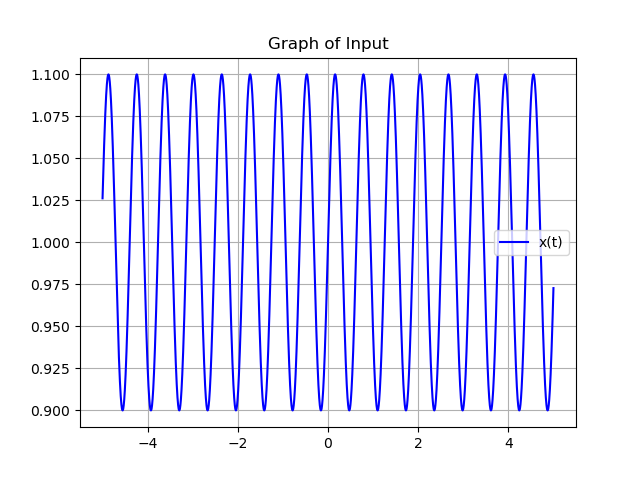
\includegraphics[width=\columnwidth]{2022/EE/37/figs/input.png}
    \caption{Input of the system, $x(t)$} 
\end{figure}
\begin{figure}[h]
    \centering
    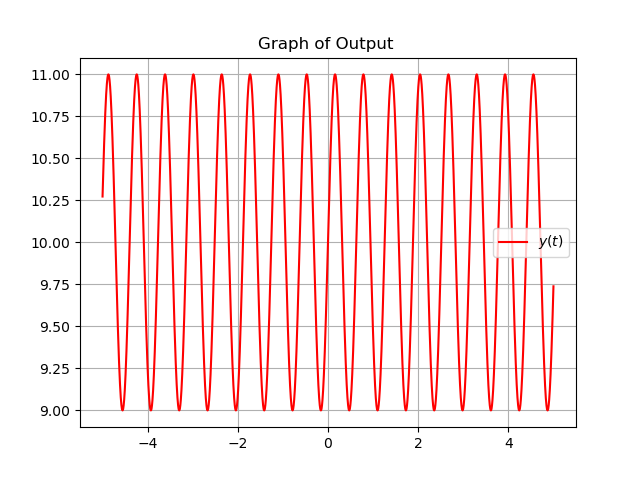
\includegraphics[width=\columnwidth]{2022/EE/37/figs/output.png}
    \caption{Output of the system, $y(t)$} 
\end{figure}
\begin{figure}[h]
    \centering
    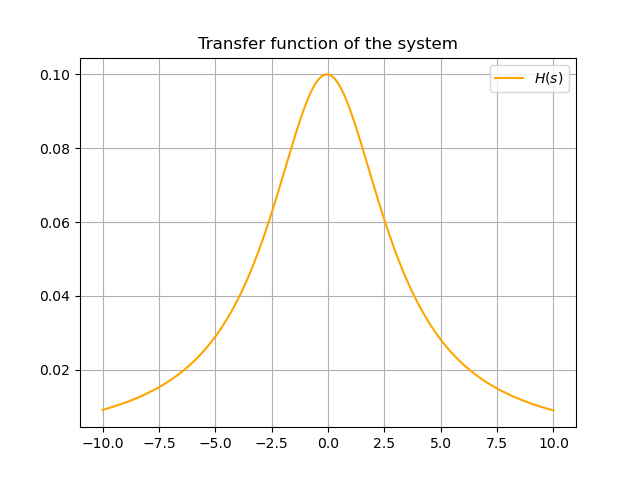
\includegraphics[width=\columnwidth]{2022/EE/37/figs/transfer.png}
    \caption{Transfer function of the system, $H(s)$} 
\end{figure}
% Properties of Laplace transform include 
% \begin{align}
%     ku\brak{t} &\system{L} \frac{k}{s}\label{37.Gate22.EE.eqn: 1}\\  
%     y\brak{t-k} & \system{L} e^{-sk} Y\brak{s} \label{37.Gate22.EE.eqn: 2}\\
%     \sin{\brak{\omega t}} &\system{L} \frac{\omega}{\omega^2 + s^2} \label{37.Gate22.EE.eqn: 3}
% \end{align}
% Taking Laplace transform of $x\brak{t}$, from \eqref{37.Gate22.EE.eqn: 1}, \eqref{37.Gate22.EE.eqn: 2} and \eqref{37.Gate22.EE.eqn: 3}
% \begin{align}
%     %a+b \sin{\brak{10t+\theta}} \system{L} 
%     1+0.1 \sin{\brak{10t}} &\system{L} \frac{1}{s} + 0.1 \frac{10}{s^2+10^2}\\
%  %   &\system{L} \frac{s^2+s+100}{s^2+100}\\
%     \implies X\brak{s} &= \frac{s^2+s+100}{s\brak{s^2+100}} \label{37.Gate22.EE.eqn: 5}
% \end{align}
% From \tabref{37.Gate22.EE.tab: 1},
% \begin{align}
%     G\brak{s}= \frac{Y\brak{s}}{X\brak{s}}=\frac{100}{s^2+0.1s+10} \\
%     \implies Y\brak{s}=X\brak{s} \brak{ \frac{100}{s^2+0.1s+10}}
% \end{align}
% From \eqref{37.Gate22.EE.eqn: 5}
% \begin{align}
%     Y\brak{s}= \frac{s^2+s+100}{s\brak{s^2+100}} \frac{100}{s^2+0.1s+10}\\
%     Y\brak{s}= 100 
% \end{align}
% Consider 
% \begin{align}
%     x(t) = x_1(t)+x_2(t)
% \end{align}
% where $x_1(t)=u(t)$ and $x_2(t)=0.1\sin{(10t)}u(t)$. 
% Since the given system is linear, 
% \begin{align}
%     y(t)=y_1(t)+y_2(t)
% \end{align}
% Where $y_1(t)$ and $y_2(t)$ are the outputs to $x_1(t)$ and $x_2(t)$ respectively.
% \begin{align}
%     y(t) \system{L} Y(s)\\
%     Y_1(s)=G(s)X_1(s)\\
%     Y_1(s)=\frac{1}{s}\brak{\frac{100}{s^2+0.1s+10}} 
% \end{align}
% By partial fractions 
% \begin{align}
%     Y_1(s)=
% \end{align}
% Consider 
% \begin{align}
%     G(s)&\system{L^{-0}}g(t)\\
%     G(s)&=\frac{100}{s^2+0.1s+10}\\
%     &=\frac{100}{(s^+0.05)^2 + 10 - (0.05)^2}\\
% \end{align}
% Let $\brak{10-\brak{0.05}^2}=a^2$ 
% \begin{align}
%     G(s)&=\frac{100}{a}\frac{a}{(s+0.05)^2+a^2}
% \end{align}
% From \eqref{37.Gate22.EE.eqn: 1}, \eqref{37.Gate22.EE.eqn: 2} and \eqref{37.Gate22.EE.eqn: 3}
% \begin{align}
%     g(t)=\frac{100}{a} e^{-0.05t}\sin{(at)}u(t)
% \end{align}
% The output of the system $y(t)$ is given by $$y(t)=x(t)*h(t)$$
% \begin{align}
%     y(t)=&\int_{-\infty}^{\infty} g(u)x(t-u) du\\
%     =&\int_{0}^{\infty} \frac{100}{a} e^{-0.05u}\sin{(au)}du \\&+ \int_{0}^{\infty} \frac{100}{a} e^{-0.05u}\sin{(au)}(0.1\sin{10(t-u)})\\
%     =&\brak{\frac{100}{a}\frac{e^{-0.05u}}{(-0.05)^2+a^2}\brak{(-0.05)\sin{au}-a\cos{au}}}_0^{\infty}\\
%     &+\int_{0}^{\infty} \frac{100}{a} e^{-0.05u}\sin{(au)}(0.1\sin{10(t-u)})\\
%     &=\frac{100}{a^2+(0.05)^2}+
% \end{align}
\end{enumerate}

 

\item A periodic function $f(x)$, with period 2, is defined as \\
   \begin{align}   
   f(x) =
   \begin{cases}
    -1-x & -1 \leq x<0 \\
     1-x &  0 <x \leq1 
   \end{cases}
   \end{align} 
   The Fourier series of this function contains \\
\begin{enumerate}[label=\Alph*.]
\item Both $\cos(n\pi x)$ and $sin(n\pi x)$ where n=1,2,3...
\item Only $\sin(n\pi x)$ where n=1,2,3...
\item Only $\cos(n\pi x)$ where n=1,2,3...
\item Only $\cos(2n\pi x)$ where n=1,2,3...  \hfill{GATE IN 2022 }
\end{enumerate} 

\solution
\let\negmedspace\undefined
\let\negthickspace\undefined
\documentclass[journal,12pt,onecolumn]{IEEEtran}
\usepackage{cite}
\usepackage{amsmath,amssymb,amsfonts,amsthm}
\usepackage{algorithmic}
\usepackage{graphicx}
\usepackage{textcomp}
\usepackage{xcolor}
\usepackage{txfonts}
\usepackage{listings}
\usepackage{enumitem}
\usepackage{mathtools}
\usepackage{gensymb}
\usepackage[breaklinks=true]{hyperref}
\usepackage{tkz-euclide} % loads  TikZ and tkz-base
\usepackage{listings}



\newtheorem{theorem}{Theorem}[section]
\newtheorem{problem}{Problem}
\newtheorem{proposition}{Proposition}[section]
\newtheorem{lemma}{Lemma}[section]
\newtheorem{corollary}[theorem]{Corollary}
\newtheorem{example}{Example}[section]
\newtheorem{definition}[problem]{Definition}
%\newtheorem{thm}{Theorem}[section] 
%\newtheorem{defn}[thm]{Definition}
%\newtheorem{algorithm}{Algorithm}[section]
%\newtheorem{cor}{Corollary}
\newcommand{\BEQA}{\begin{eqnarray}}
\newcommand{\EEQA}{\end{eqnarray}}
\newcommand{\define}{\stackrel{\triangle}{=}}
\theoremstyle{remark}
\newtheorem{rem}{Remark}
%\bibliographystyle{ieeetr}
\begin{document}
%
\providecommand{\pr}[1]{\ensuremath{\Pr\left(#1\right)}}
\providecommand{\prt}[2]{\ensuremath{p_{#1}^{\left(#2\right)} }}        % own macro for this question
\providecommand{\qfunc}[1]{\ensuremath{Q\left(#1\right)}}
\providecommand{\sbrak}[1]{\ensuremath{{}\left[#1\right]}}
\providecommand{\lsbrak}[1]{\ensuremath{{}\left[#1\right.}}
\providecommand{\rsbrak}[1]{\ensuremath{{}\left.#1\right]}}
\providecommand{\brak}[1]{\ensuremath{\left(#1\right)}}
\providecommand{\lbrak}[1]{\ensuremath{\left(#1\right.}}
\providecommand{\rbrak}[1]{\ensuremath{\left.#1\right)}}
\providecommand{\cbrak}[1]{\ensuremath{\left\{#1\right\}}}
\providecommand{\lcbrak}[1]{\ensuremath{\left\{#1\right.}}
\providecommand{\rcbrak}[1]{\ensuremath{\left.#1\right\}}}
\newcommand{\sgn}{\mathop{\mathrm{sgn}}}
\providecommand{\abs}[1]{\left\vert#1\right\vert}
\providecommand{\res}[1]{\Res\displaylimits_{#1}} 
\providecommand{\norm}[1]{\left\lVert#1\right\rVert}
%\providecommand{\norm}[1]{\lVert#1\rVert}
\providecommand{\mtx}[1]{\mathbf{#1}}
\providecommand{\mean}[1]{E\left[ #1 \right]}
\providecommand{\cond}[2]{#1\middle|#2}
\providecommand{\fourier}{\overset{\mathcal{F}}{ \rightleftharpoons}}
\newenvironment{amatrix}[1]{%
  \left(\begin{array}{@{}*{#1}{c}|c@{}}
}{%
  \end{array}\right)
}
%\providecommand{\hilbert}{\overset{\mathcal{H}}{ \rightleftharpoons}}
%\providecommand{\system}{\overset{\mathcal{H}}{ \longleftrightarrow}}
	%\newcommand{\solution}[2]{\textbf{Solution:}{#1}}
\newcommand{\solution}{\noindent \textbf{Solution: }}
\newcommand{\cosec}{\,\text{cosec}\,}
\providecommand{\dec}[2]{\ensuremath{\overset{#1}{\underset{#2}{\gtrless}}}}
\newcommand{\myvec}[1]{\ensuremath{\begin{pmatrix}#1\end{pmatrix}}}
\newcommand{\mydet}[1]{\ensuremath{\begin{vmatrix}#1\end{vmatrix}}}
\newcommand{\myaugvec}[2]{\ensuremath{\begin{amatrix}{#1}#2\end{amatrix}}}
\providecommand{\rank}{\text{rank}}
\providecommand{\pr}[1]{\ensuremath{\Pr\left(#1\right)}}
\providecommand{\qfunc}[1]{\ensuremath{Q\left(#1\right)}}
	\newcommand*{\permcomb}[4][0mu]{{{}^{#3}\mkern#1#2_{#4}}}
\newcommand*{\perm}[1][-3mu]{\permcomb[#1]{P}}
\newcommand*{\comb}[1][-1mu]{\permcomb[#1]{C}}
\providecommand{\qfunc}[1]{\ensuremath{Q\left(#1\right)}}
\providecommand{\gauss}[2]{\mathcal{N}\ensuremath{\left(#1,#2\right)}}
\providecommand{\diff}[2]{\ensuremath{\frac{d{#1}}{d{#2}}}}
\providecommand{\myceil}[1]{\left \lceil #1 \right \rceil }
\newcommand\figref{Fig.~\ref}
\newcommand\tabref{Table~\ref}
\newcommand{\sinc}{\,\text{sinc}\,}
\newcommand{\rect}{\,\text{rect}\,}
%%
%	%\newcommand{\solution}[2]{\textbf{Solution:}{#1}}
%\newcommand{\solution}{\noindent \textbf{Solution: }}
%\newcommand{\cosec}{\,\text{cosec}\,}
%\numberwithin{equation}{section}
%\numberwithin{equation}{subsection}
%\numberwithin{problem}{section}
%\numberwithin{definition}{section}
%\makeatletter
%\@addtoreset{figure}{problem}
%\makeatother

%\let\StandardTheFigure\thefigure
\let\vec\mathbf


\bibliographystyle{IEEEtran}
\title{ GATE IN-13 2022}
\author{EE23BTECH11011- Batchu Ishitha$^{*}$% <-this % stops a space
}
\maketitle




\bigskip

\renewcommand{\thefigure}{\theenumi}
\renewcommand{\thetable}{\theenumi}
%\renewcommand{\theequation}{\theenumi}

Q: A periodic function $f(x)$, with period 2, is defined as \\
   \begin{align}   
   f(x) =
   \begin{cases}
    -1-x & -1 \leq x<0 \\
     1-x &  0 <x \leq1 
   \end{cases}
   \end{align} 
   The Fourier series of this function contains \\
\begin{enumerate}[label=\Alph*.]
\item Both $\cos(n\pi x)$ and $sin(n\pi x)$ where n=1,2,3...
\item Only $\sin(n\pi x)$ where n=1,2,3...
\item Only $\cos(n\pi x)$ where n=1,2,3...
\item Only $\cos(2n\pi x)$ where n=1,2,3...  \hfill{GATE IN 2022 }
\end{enumerate} 

\solution

\begin{table}[!ht]    
    \centering
    
\begin{tabular}{|c|c|l|}
\hline
Parameter  & Value & Description   \\             
\hline
$y(0)$     & $0$   & Initial displacement  \\     
 \hline
$y'(0)$    & $0$   & First derivative at $t=0$  \\
 \hline
$y''(0)$   & $0$   & Second derivative at $t=0$ \\
 \hline
$y'''(0)$  & $0$   & Third derivative at $t=0$  \\
 \hline
\end{tabular}


    \caption{Input Parameters}
    \label{table:ishitha.g22.in.13.t1}
\end{table}

The complex exponential Fourier Series of $f\brak{x}$ is,
\begin{align}
    f\brak{x}&=\sum_{n=-\infty}^{\infty}c(n)e^{jn\omega x}\\
    \implies c(n)&=\frac{1}{2L}\int_{-L}^{L}f\brak{x}e^{-jn\omega x}\;dx\\
\end{align}    

For $n\neq 0$;
\begin{align}
c(n) &= \frac{1}{2} \int_{-1}^{1} f(x) e^{-jn\omega x} \, dx \\
&= \frac{1}{2} \brak{ \int_{-1}^{0}\brak{-1-x}e^{-jn\omega x} \, dx +  \int_{0}^{1}\brak{+1-x}e^{-jn\omega x} \, dx } \\
&= \frac{1}{2} \brak{-\int_{-1}^{0}e^{-jn\omega x} \, dx -\int_{-1}^{1}xe^{-jn\omega x} \, dx + \int_{0}^{1}e^{-jn\omega x} \, dx} \\
&= \frac{1}{2} \sbrak{\frac{-1}{jn\omega }\sbrak{-\brak{1 - e^{+jn\omega }} + \brak{e^{-jn\omega } -1}} -\int_{-1}^{1}xe^{-jn\omega x} \, dx} \\
&= \frac{1}{2} \sbrak{\frac{-1}{jn\omega }\sbrak{-2 +e^{+jn\omega } + e^{-jn\omega }} +\brak{\frac{e^{-jn\omega x}}{jn\omega }\sbrak{x + \frac{1}{jn\omega }}}_{-1}^{1}} \\
&= \frac{-1}{jn\omega }\sbrak{-1 + \cos(n\omega )} + \frac{1}{2(jn\omega )^2}\sbrak{\brak{e^{-jn\omega }}\brak{1+jn\omega }- \brak{e^{jn\omega } }\brak{-jn\omega +1}} \\
\implies c\brak{n}&= \frac{-1}{(jn\omega )^2}\sbrak{-jn\omega  + j \sin(n\omega )}
\end{align} 

For $n=0$;
\begin{align}
c(0) &= \frac{1}{2} \int_{-1}^{1} f(x) \, dx \\
&=  \frac{1}{2} \sbrak {\int_{-1}^{0} \brak{-1-x} \, dx + \int_{0}^{1} \brak{1-x} \, dx } \\
&= \frac{1}{2} \sbrak{ \brak{-x-\frac{x^2}{2}}_{-1}^{0} + \brak{x-\frac{x^2}{2}}_{0}^{1}} \\
&= \frac{1}{2} \sbrak{0-1+\frac{1}{2} +1 -\frac{1}{2} -0} \\
\implies c(0)&= 0
\end{align}


The trigonometric Fourier Series of $f\brak{x}$ is,
\begin{align}
    f\brak{x}=a(0)+\sum_{n=1}^{\infty}\cbrak{a(n)\cos\brak{n\omega x}+b(n)\sin\brak{n\omega x}}
\end{align}

Finding the Fourier Coefficient $a_0$,
\begin{align}
    a(0)&=c(0)\\
    \implies a(0)&= 0
\end{align}

Finding the Fourier Coefficients $a(n)$,
\begin{align}
    a(n)&=\frac{1}{L}\int_{-L}^{L}f(x)\cos\brak{n\omega x}\;dx, n \geq 0 \\
    &= \frac{1}{L}\int_{-L}^{L}f(x)\brak{e^{-jn\omega x}+e^{jn\omega x}} \; dx \\
 \implies a(n)   &= c(n) + c(-n) \\
 \implies a(n)&= 0 \\
\end{align}  
  
Finding the Fourier Coefficients $b(n)$,
\begin{align}
    b_n&=\frac{1}{L}\int_{-L}^{L}f(x)\sin\brak{n\omega x}\;dx, n \geq 0 \\
    &= \frac{1}{L}\int_{-L}^{L}f(x)j\brak{e^{-jn\omega x}-e^{jn\omega x}} \; dx \\
   \implies b(n) &= j\brak{c\brak{n} - c\brak{-n}} \\
   \implies b(n)&= \frac{-2}{(n\omega )^2}\sbrak{-n\omega +  \sin(n\omega)} 
\end{align}  

$\implies$ The trigonometric Fourier Series of $f\brak{x}$ is,
\begin{align}
 f\brak{x} &=\sum_{n=1}^{\infty}\cbrak{0+ 0 +b(n)\sin\brak{n\omega x}} \\
 f\brak{x} &=\sum_{n=1}^{\infty}\cbrak{\frac{-2}{(n\omega )^2}\sbrak{-n\omega +  \sin(n\omega)} \sin\brak{n\omega x}} \\
 f\brak{x} &=\sum_{n=1}^{\infty}\cbrak{\frac{-2}{(n\pi )^2}\sbrak{-n\pi +  \sin(n\pi)} \sin\brak{n\pi x}} \\
  f\brak{x} &=\sum_{n=1}^{\infty}\cbrak{\frac{2}{n\pi } \sin\brak{n\pi x}}
 \end{align}

 $\therefore$ The Fourier series of this function contains only $\sin(n\pi x)$ where n=1,2,3...
 
 \begin{figure}[!ht]
    \centering
     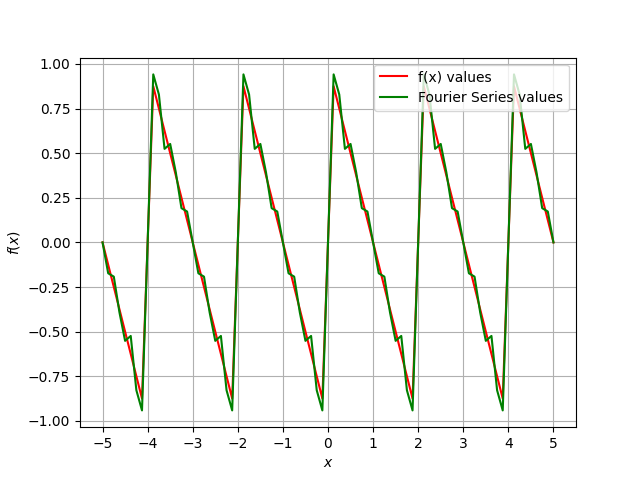
\includegraphics[width=\columnwidth]{./figs/f.png}
    \caption{}    
    \label{fig:ishitha.g22.in.13.f1}
\end{figure}
 

\end{document}

\item  A Simple closed path C in the Complex Plane is shown in the figure.
 \begin{align*}
        \oint_C \frac{2^z}{z^2-1}dz=-\jmath \pi A
 \end{align*}
 Where $\jmath=\sqrt{-1}$, Then find the value of A is \rule{1cm}{0.15mm}(Rounded of to two decimals)
\begin{figure}[h!]
    \centering
    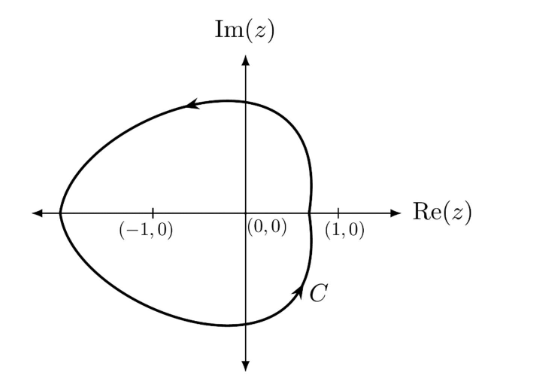
\includegraphics[width = \columnwidth]{2022/EC/32/figs/fig1.png}
\end{figure}
\hfill{(GATE 2022 EC)}\\
\solution 
\input{2022/EC/32/EC_32.tex}
\end{enumerate}
